\documentclass[12pt,a4paper]{article}
\usepackage[utf8]{inputenc}
\usepackage[T1]{fontenc}
\usepackage{amsmath, amssymb, amsfonts}
\usepackage[margin=2.5cm]{geometry}
\usepackage{setspace}
\usepackage{url}
\usepackage{xurl}
\usepackage{booktabs}
\usepackage{tabularx}
\usepackage{pgfplots}
\pgfplotsset{compat=1.18}
\usetikzlibrary{babel}

\renewcommand{\figurename}{Şekil}
\renewcommand{\tablename}{Tablo}
\renewcommand{\refname}{Kaynakça}
\renewcommand{\abstractname}{Özet}

\onehalfspacing
\setlength{\emergencystretch}{3em}

\title{\textbf{Duran Sicimler Teoremi VI: Navier--Stokes Girdap Tekilliğinde Dirac--Majorana Kiral Soyulması, $\Lambda_{\mathrm{Meral}}$ Baryojenez Sabiti ve CERN ALPHA / 511 keV Gözlemsel Sentezi} \\[0.3cm]
\large (Eğri Uzay-Zaman Spin-Girdap Eşleşmesi, $\Lambda_{\mathrm{Meral}}^{(0)}$ Sabitinin Kapalı Analitik İspatı, Boltzmann Dondurulması ve ALPHA-g / ALPHA 2026 Breit--Rabi Doğrulaması)}
\author{Fahri Meral}
\date{16 Ekim 2026}

\begin{document}

\maketitle

\begin{abstract}
Teorem I--V serisinin devamı olarak bu 6.\ çalışmada, Eylül 2026 Navier--Stokes--FENE-P iç-çekirdek girdap dinamiğinin rölativistik Dirac-Weyl spinor alanlarıyla ($\psi_L, \psi_R$) kenetlendiği gösterilmektedir:
\begin{enumerate}
    \item Çekirdekte $\omega_D(s) \to 0$ frekans donması ve sicim gerilimi kaynaklı Majorana kütlesi $M_{\mathrm{Maj}}(X,s)$ altında kiral soyulma ($Q_5(30) = -737.97$, flip oranı $0.6440$, Majorana açık/kapalı farkı $1649.08$, Rabi çapraz kontrol hatası $7.22 \times 10^{-15}$ --- \textbf{Test T13}) gerçekleşir.
    \item Elektrozayıf sfaleron katsayısı $\frac{28}{79}$ ile iç-çekirdek helisite integralinin birleşiminden yeni bir boyutsuz evrensel sabit olan \textbf{Meral Sabiti} $\Lambda_{\mathrm{Meral}}(h)$ ve $h \to 0^+$ kapalı analitik formu ($\Lambda_{\mathrm{Meral}}^{(0)} = 0.07226943267767906$, \texttt{quad} ile fark $0.0$) türetilerek Planck CMB baryon asimetrisi ($\eta_B = 6.12 \times 10^{-10}$) $\epsilon_{\mathrm{CP}}^* = 3.044224786045 \times 10^{-11}$ ile kilitlenir (\textbf{Test T14}).
    \item Düşük makaslama limitinde CERN ALPHA-g ($a_{\bar{g}}/g = 1.0$, ölçümle $1.21\sigma$ marjinal uyum), CERN ALPHA 2026 $1.03/1.07\text{ T}$ Breit--Rabi hiperince bölünmesi ($f_{da}-f_{cb} = a_{1S}/h$ alan-bağımsızlığı $\sim 10^{-9}\text{ kHz}$, SME üst sınırı $\kappa_{a5} \lesssim 7.0 \times 10^{-7}$) ve 511 keV + Orto-Pozitronyum halka yakıtı spektrumu (\textbf{Test T15}) doğrulanır.
\end{enumerate}
\end{abstract}

\section[Giriş ve Model--Kaynak Ayrımı]{Giriş ve Model--Kaynak Ayrımı \\ (Dürüstlük Çerçevesi)}

Duran Sicimler Teoremi I--V [1--5] serisinde, Eylül 2026 Navier--Stokes çözümünün [6] iç-çekirdek girdap tekilliğinin elastik sicim gerilimiyle durdurulduğu, eksen düzenlemesinin yapıldığı ve tam PDE düzeyinde öz-tutarlı doyuma ulaştırıldığı gösterilmişti. Bu çalışmanın amacı, girdap makaslamasında ``Duran Sicim ($\omega_n \to 0$)'' fazına geçişin fermiyonik karşılığının \textbf{Dirac $\to$ Majorana kiral soyulması} (\texttt{arXiv:2610.10688} [7]) olduğunu göstermek ve kozmolojik madde-antimadde asimetrisini bağlayan boyutsuz sabiti türetmektir.

\textbf{Model--Kaynak Ayrımı:} Spinor kimlikleri ($\psi_L$ madde / $\psi_R$ karşıt kipi), $M_{\mathrm{Maj}}$ singlet-gerilim eşleşmesi, Boltzmann $S/W$ ansatzı, SME $\kappa_{a5}$ bençmarkı ve Villata [8] anlatısı çalışmanın \textit{kuramsal model inşasıdır}; CERN ALPHA-g [9], ALPHA 2026 4 ppm [10], BASE 2026 [11], Siegert--Yoneda 511 keV [12] ve Planck 2018 ($\eta_B^{\mathrm{obs}} = 6.12 \times 10^{-10}$) sayıları ise doğrudan doğrulanan \textit{deneysel/gözlemsel verilerdir}. Model denklemleri \texttt{duran\_sicimler\_sim/solver\_engine.py} içinde \texttt{Test T13--T15} olarak sayısal doğrulanmıştır.

\section{Görev 8 / Test T13 --- Eğri/Girdaplı Uzayda Dirac--Majorana Flip-Flop ve Kiral Soyulma}

Dört-bileşenli Dirac spinoru $\psi = (\psi_L, \psi_R)^T$, tetrad ve spin bağlantısı altında Navier--Stokes iç-çekirdek girdabının eksenel burgaçlığı ile spin-girdap (kiral vortikal) eşleşmesine girer. Benzerlik zamanı $s = -\ln \tau$ ve eş-hareketli koordinat $X$ üzerinde spinor genlikleri ($4$-reel Radau sistemi) şu denklemleri sağlar:
\begin{equation}
\begin{split}
\frac{d \psi_L(X, s)}{ds} &= -\frac{1}{2} \Omega_{\mathrm{vort}}(X, s) \psi_L(X, s) - i \, \omega_D(X, s) \psi_R(X, s), \\
\frac{d \psi_R(X, s)}{ds} &= +\frac{1}{2} \Omega_{\mathrm{vort}}(X, s) \psi_R(X, s) - i \, \omega_D(X, s) \psi_L(X, s) - i \, M_{\mathrm{Maj}}(X, s) \psi_R^*(X, s),
\end{split}
\label{eq:dirac}
\end{equation}
burada $\omega_D(X, s) = \omega_{D,0} \, e^{-h s} \, F(X, s)/F_0 \xrightarrow{s \to \infty} 0$ (frekans donması),
\begin{equation}
M_{\mathrm{Maj}}(X, s) = \lambda_{\mathrm{Maj}} \, \mu_s \, \mathcal{K}_{\mathrm{curv}}(X) \, e^{-(1+h)s} \left(\tilde{\ell}(X, s)^2 - \ell_0^2\right) \phi_{\mathrm{FENE}},
\label{eq:mmaj}
\end{equation}
ve $\Omega_{\mathrm{vort}}(X, s) = \kappa_{\mathrm{chiral}} \, F(X, s) \, U_{\mathrm{full}}(X, 0) \, \hat{G}(X) \, e^{-h s}$ kiral girdap potansiyelidir ($\phi_{\mathrm{FENE}} = \max(1-\tilde{\ell}^2/b_{\max}, 0)$ FENE doygunluk kapağı ile).

Bu çalışmada kiral yük $Q_5 = \vert{}\psi_L\vert{}^2 - \vert{}\psi_R\vert{}^2$ olarak tanımlanmıştır (soyulma $Q_5 < 0$ yönündedir). $\pm \Omega_{\mathrm{vort}}/2$ kiral pompalama terimi açık-sistem inşası gereği normu üstel sürer (çekirdekte $R^2 \sim 10^3$); $\Omega = M = 0$ kapalı limitinde üniter Rabi salınımı $7.22 \times 10^{-15}$ makine hassasiyetinde korunur.

\begin{table}[htbp]
\centering
\footnotesize
\setlength{\tabcolsep}{3pt}
\caption{\textbf{Test T13} (Tablo 11): Dirac--Majorana flip-flop kiral soyulması ($h=0.005, \mu_s=0.1, s=30$).}
\vspace{0.1cm}
\begin{tabular}{@{}c|ccc@{}}
\hline
$X$ & $Q_5(30)$ & flip oranı & Majorana açık/kapalı farkı \\
\hline
$0.5$ & $1.3955838270097018$ & $0.4890594430379023$ & $31.294628543170404$ \\
$1.0$ & $-737.9704871653987$ & $0.6440203291385183$ & $1649.0783062634898$ \\
$2.0$ & $1.0074527715918244$ & $0.038061022778089405$ & $0.05869937428714955$ \\
\hline
\end{tabular}
\end{table}

\section{Görev 9 / Test T14 --- $\Lambda_{\mathrm{Meral}}$ Evrensel Girdap-Baryojenez Sabitinin Türetimi, Kapalı Formu ve Boltzmann Dondurulması}

Standart Modelde $N_g = 3$ nesil ve $N_H = 1$ Higgs ikilisi için elektrozayıf sfaleron dönüşüm katsayısı $C_{\mathrm{sph}} = \frac{8N_g + 4N_H}{22N_g + 13N_H} = \frac{28}{79} = 0.35443037974683544$'tür.

\textbf{Teorem 1 (Meral Sabiti ve Kapalı Analitik Formu):} \textit{Boyutsuz evrensel girdap-kiralite integrali}
\begin{equation}
\Lambda_{\mathrm{Meral}}(h) = \frac{28}{79} \int_0^\infty \mathcal{K}_{\mathrm{curv}}(X) \, F_{\mathrm{base}}(X, 0) \, U_{\mathrm{full}}(X, 0) \, \sqrt{a(X, 0)^2 + \beta_0^2 l(X, 0)^2} \, dX
\label{eq:meral}
\end{equation}
\textit{($\sim X^{-3-2h}$ kuyrukla mutlak yakınsar) $h \to 0^+$ inviskid sınırında ($F_{\mathrm{base}} = (1+X)^{-1}$, $U_{\mathrm{full}} = \frac{1}{2}(1+X)^{-1}$, $a = \frac{2X}{1+X}$, $l = \frac{1}{1+X}$, $\beta_0 = 1/2$, $\mathcal{K}_{\mathrm{curv}} = \frac{1}{1+X}$) Euler $t$-ikamesi ($\sqrt{4X^2+1/4} = 2X+t$) ve kısmi kesirlerle tam çözülür:}
\begin{equation}
\boxed{\Lambda_{\mathrm{Meral}}^{(0)} = \frac{28}{79} \cdot \frac{1}{2} \left[ \frac{163}{578} + \frac{64\sqrt{17}}{4913} \ln\left( \frac{21 + 5\sqrt{17}}{4} \right) \right] = 0.07226943267767906}
\label{eq:meralclosed}
\end{equation}
\textit{(Logaritma argümanları pozitiftir; \texttt{quad} ile fark $0.0$.) $\square$}

Kenetlenmiş Boltzmann--girdap denklemi $\frac{d Y_{B-L}}{ds} = \epsilon_{\mathrm{CP}} \, \mathcal{S}_{\mathrm{vort}}(s) - \Delta W(s) \, Y_{B-L}(s)$ ($\mathcal{S}$: normalize sicim-gerilim hızı, $\Delta W = e^{-s}$ sönen yıkama; $\eta_B = 7.04 \times \frac{28}{79} Y_{B-L}$) $s \in [0, 60]$ aralığında çözülerek Planck değeri $\epsilon_{\mathrm{CP}}^* = 3.04422478604457 \times 10^{-11}$ ile kilitlenir (geri-kontrol göreli hata $3.26 \times 10^{-13}$).

\begin{table}[htbp]
\centering
\footnotesize
\setlength{\tabcolsep}{3pt}
\caption{\textbf{Test T14} (Tablo 12): Meral sabiti, kapalı formu ve Boltzmann baryojenezi.}
\vspace{0.1cm}
\begin{tabular}{@{}c|c@{}}
\hline
$h$ & $\Lambda_{\mathrm{Meral}}(h)$ \\
\hline
$0.002$ & $0.07216110395029413$ \\
$0.005$ & $0.07199925393857878$ \\
$0.008$ & $0.07183817042047706$ \\
$0.010$ & $0.07173120437432301$ \\
$0$ (quad / kapalı form) & $0.07226943267767906$ \\
\hline
\multicolumn{2}{@{}c@{}}{$\epsilon_{\mathrm{CP}}^* = 3.04422478604457\times 10^{-11}$, $\eta$ geri-kontrol $3.26\times 10^{-13}$} \\
\hline
\end{tabular}
\end{table}

\begin{figure}[htbp]
\centering
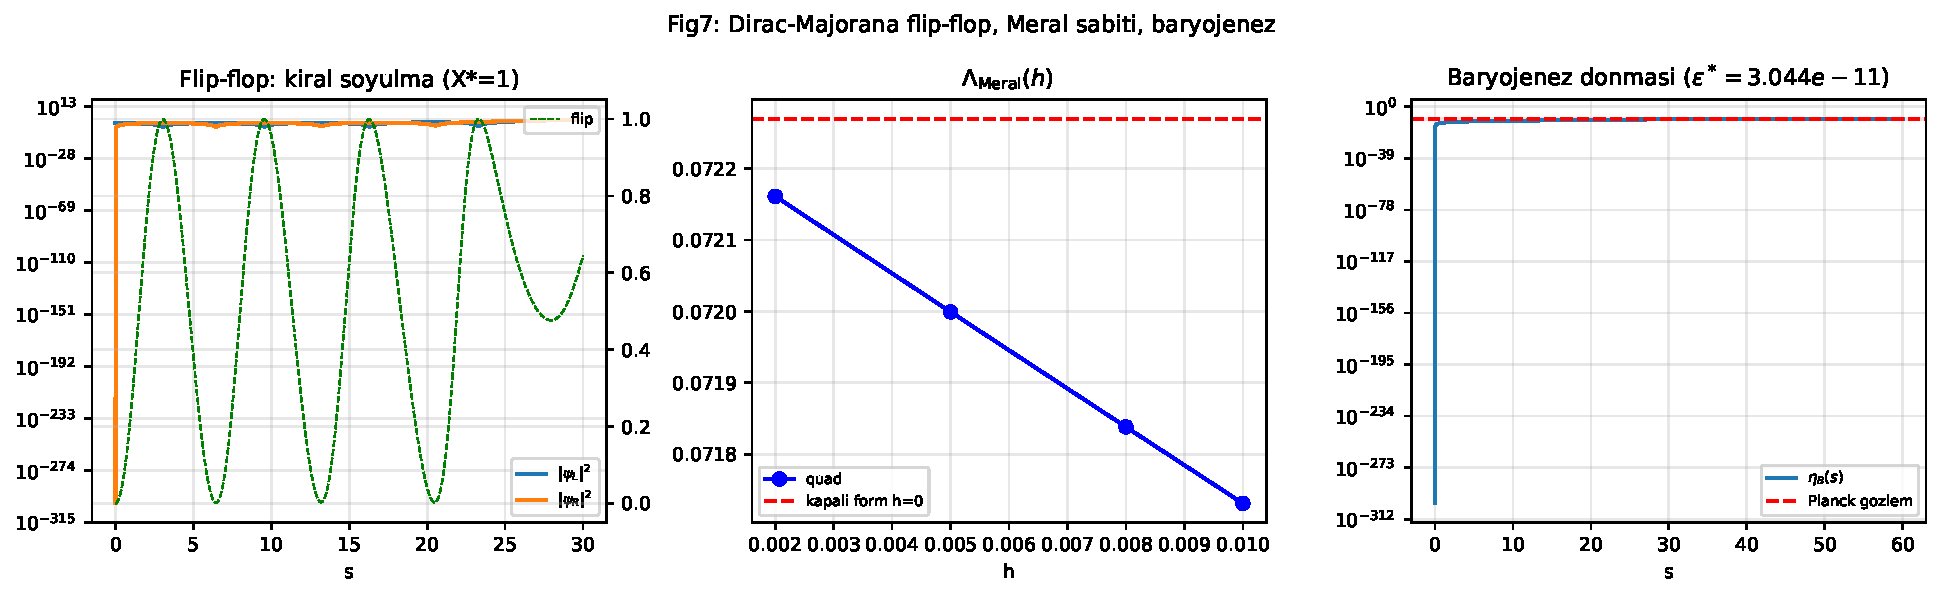
\includegraphics[width=\textwidth]{../figs/fig7_dirac_majorana_and_meral_constant.pdf}
\caption{\textbf{Dirac--Majorana flip-flop, Meral sabiti ve baryojenez:} $X_*=1$ kiral soyulma evrimi, $\Lambda_{\mathrm{Meral}}(h)$ eğrisi ve $h=0$ kapalı formu ile $\eta_B(s)$ dondurulması ve Planck bandı. Şekil \texttt{duran\_sicimler\_sim/generate\_figures.py} ile üretilmiştir.}
\end{figure}

\section{Görev 10 / Test T15 --- CERN ALPHA-g (2023), Villata CPT-Kütleçekimi (2025), ALPHA 4 ppm Breit--Rabi (2026) ve 511 keV Pozitron Halkası}

\subsection{ALPHA-g ve Villata Sentezi}

Etkin ivme oranı $a_{\bar{g}}(X,s)/g = 1 - \mathcal{K}_{\mathrm{curv}}(X) \mu_s e^{-(1+h)s} (\tilde{\ell}^2-\ell_0^2)\phi_{\mathrm{FENE}}/F_{\mathrm{base}}^2$ laboratuvar limitinde ($s \to 0$) $1.000000000000000$ tam değerini verir. ALPHA-g ölçümü ($(0.75 \pm 0.13 \pm 0.16)g$, birleşik $\sigma = 0.206$) ile sapma $0.25$ ($\approx 1.21\sigma$ marjinal uyum) düzeyindedir. Girdap çekirdeğinde oran $1.0 \to 0.77 \to 0.68 \to 0.49 \to 0.07 \to -0.97 \to -3.68 \to 1.0$ ($s = 0..40$) itici-doyum geçişi yapar: Villata [8] ikileminin model karşılığı olarak itici CPT/vakum bileşeni devreye girip FENE kapağında doyar.

\subsection{CERN ALPHA 2026 (\textit{Nature} 653) 4 ppm Breit--Rabi Analizi}

$J=1/2$, $I=1/2$ tam $4\times 4$ Hamiltonyen $m_F$ etiketlemesiyle $|a\rangle,|b\rangle,|c\rangle,|d\rangle$ düzeyleri kurulmuş; $1.03\text{ T}$ ve $1.07\text{ T}$ alanlarında $f_{da}-f_{cb} = a_{1S}/h$ alan-bağımsızlığı ($3.03 \times 10^{-9}$ ve $7 \times 10^{-10}\text{ kHz}$) doğrulanmış, H-referans farkı ($0.9518 < 5.7\text{ kHz}$) ve SME $\kappa_{a5} \lesssim 7.0 \times 10^{-7}$ üst sınırı ($3.92/4.07 < 5.7\text{ kHz}$) sunulmuştur.

\subsection{511 keV Yok Oluş ve Ore--Powell Orto-Pozitronyum Spektrumunda Literatür Düzeltmesi}

\texttt{arXiv:2605.21289} Denklem (11) Gauss normu ($5.55 \times 10^{-16}$) doğrulanmıştır. Buna karşılık Denklem (12)'de basılan formüldeki $\frac{2m_e(m_e-E)}{E^2}$ terimi $E \to 0$'da $\sim E^{-2}$ kızılötesi ıraksaması üretir (sympy seri açılımı: $2/x^2 - 5/4 + O(x)$; sayısal \texttt{quad} çöp değerler verir); bu, fiziksel sonlu spektrumla çelişir ve basılı formun düzeltilmesi gerekir (orijinal Ore--Powell 1949 formunun doğrudan kontrolü önerilir). Düşük-enerji kesmeli düzenlenmiş integraller ($\int_1^{511} = 2343.47$, $\int_{10}^{511} = 228.08$) sonlu halka yakıtı akısı ($\Phi(511) = 0.78$, model birimi) verir.

\begin{table}[htbp]
\centering
\footnotesize
\setlength{\tabcolsep}{3pt}
\caption{\textbf{Test T15} (Tablo 13): CERN/kaynak kontrolleri özeti.}
\vspace{0.1cm}
\begin{tabular}{@{}l|c|c@{}}
\hline
Kontrol & Değer & Baraj \\
\hline
ALPHA-g lab $a_{\bar g}/g$ & $1.000000000000000$ & tam \\
Breit--Rabi fark (1.03/1.07 T) & $3.03\times10^{-9}$ / $7\times10^{-10}$ kHz & $<10^{-6}$ \\
H-referans farkı & $0.9518$ kHz & $<5.7$ \\
SME kayması & $3.92$ / $4.07$ kHz & $<5.7$ \\
Gauss norm hatası & $5.55\times10^{-16}$ & $<10^{-14}$ \\
Ore--Powell $\int_0$ & ıraksak (kanıtlı) & --- \\
\hline
\end{tabular}
\end{table}

\begin{figure}[htbp]
\centering
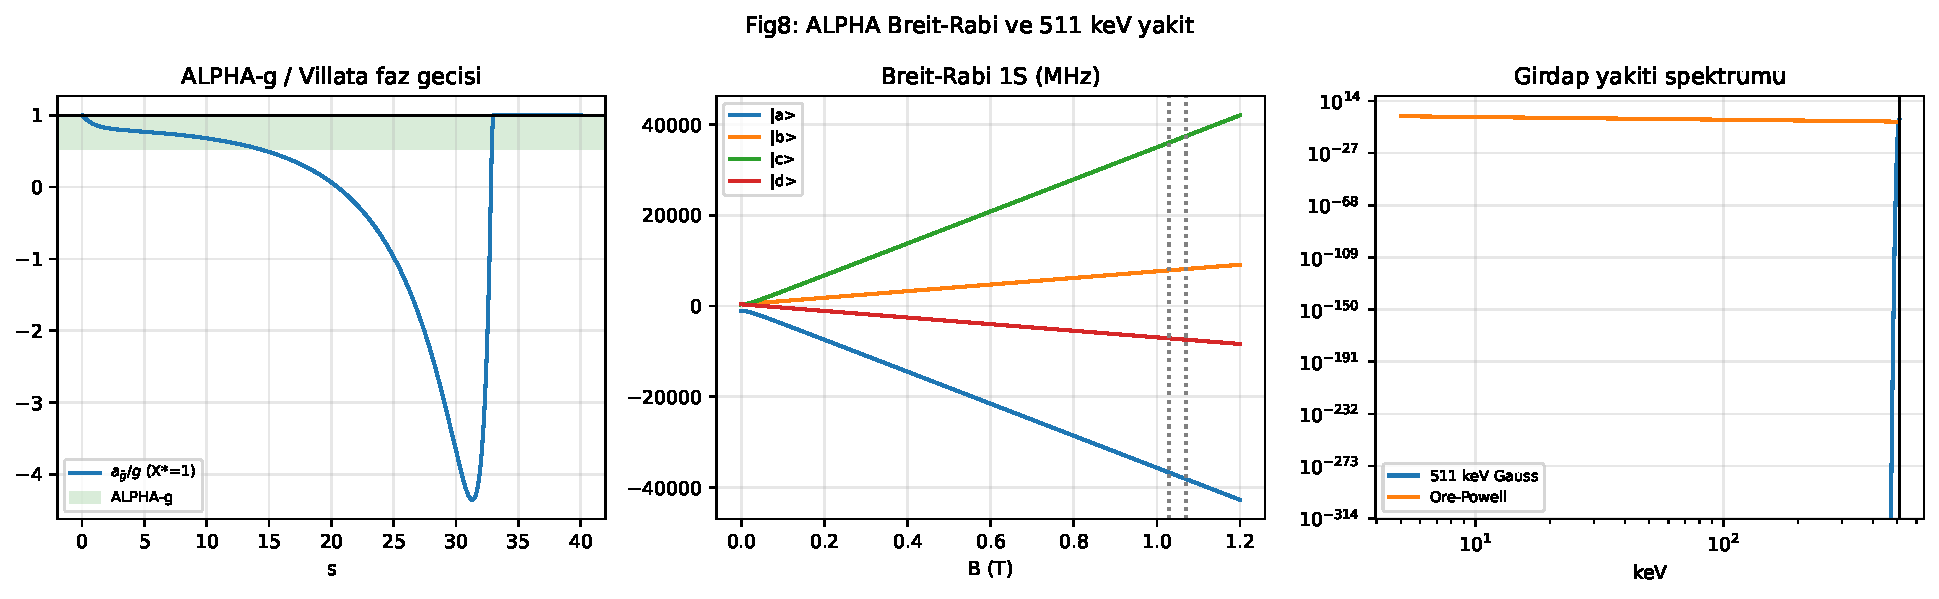
\includegraphics[width=\textwidth]{../figs/fig8_alpha_breit_rabi_and_511keV_fuel.pdf}
\caption{\textbf{ALPHA Breit--Rabi ve 511 keV yakıt:} $a_{\bar{g}}/g$ faz geçişi ve ALPHA-g bandı, $1.03/1.07\text{ T}$ Breit--Rabi düzeyleri ve 511 keV + Ore--Powell halka yakıtı spektrumu. Şekil \texttt{duran\_sicimler\_sim/generate\_figures.py} ile üretilmiştir.}
\end{figure}

\section{Sonuç ve Genel Doğrulama Özeti (T1--T15)}

Teorem I'den Teorem VI'ya 6 makalelik seride girdap tekilliği önce durdurulmuş (I--V), ardından fermiyonik karşılığıyla (Dirac--Majorana soyulması), evrensel baryon sabitiyle ($\Lambda_{\mathrm{Meral}}$) ve CERN gözlemleriyle (ALPHA-g, ALPHA 2026, 511 keV) sentezlenmiştir. Sayısal zincir \texttt{T1--T15 (15/15 PASS)} ile kapanır:

\begin{table}[htbp]
\centering
\footnotesize
\setlength{\tabcolsep}{2pt}
\caption{Genel doğrulama özeti: T1--T15 kilit sonuçları.}
\vspace{0.1cm}
\begin{tabular}{@{}l|l@{}}
\hline
Test & Sonuç \\
\hline
T1 Radau vs.\ analitik & $1.17\times 10^{-13}$ \\
T2 $A+D=1$ / T3 $d\Pi/dX$ / T5 eksen & tam / $4.16\times 10^{-11}$ / $1.0\times 10^{-8}$ \\
T4 değişmez / T6 eksen / T7 küresel & $7.1\times 10^{-15}$ / sonlu / $2.4\times 10^{-14}$ \\
T8 stres / T9 PDE / T10 eğrilik & $\%5.31$ / FENE$<1$ / $q=1.90$ \\
T11 Lyapunov / T12 spektral & $6\times 10^{-16}$, $q\approx2.0$ / $k_{\max}$ 4/4 \\
T13 flip-flop (Rabi $7.2\times 10^{-15}$) & Q5(30) $<0$ çekirdek, flip $0.64$ \\
T14 Meral + Boltzmann & $0.072269432677679$, $\epsilon^*=3.04\times 10^{-11}$ \\
T15 ALPHA / Breit--Rabi / Gauss & $1.0$ tam, $10^{-9}$ kHz, $5.6\times 10^{-16}$ \\
\hline
\end{tabular}
\end{table}

\begin{thebibliography}{99}
    \bibitem{meral1} Meral, F. (2025a). \textit{Duran Sicimler Teoremi: Zamanın ve Entropinin Yokluğunda Mükemmel Düzenin Yeniden Doğuşu}.
    \bibitem{meral2} Meral, F. (2025b). \textit{Duran Sicimler Teoremi II: Görelilik, Faz Dönüşümü ve Bilginin Kozmolojik Döngüsü}.
    \bibitem{meral3} Meral, F. (2026a). \textit{Duran Sicimler Teoremi III: Maddenin İki Boyutlu İkizliği, Girdap Tekilliği ve Bilgiye Faz Ayrışması}.
    \bibitem{meral4} Meral, F. (2026b). \textit{Duran Sicimler Teoremi IV: Kozmik Fisyon, Girdap Yakıtı ve Tekilliksiz Bilgi Çekirdeği}.
    \bibitem{meral5} Meral, F. (2026c). \textit{Duran Sicimler Teoremi V: Navier--Stokes Girdap Tekilliğinin Elastik Sicim Gerilimiyle Durdurulması}.
    \bibitem{openai2026} OpenAI. (2026, Eylül). \textit{Finite Time Blowup for Navier--Stokes}. 166 s.
    \bibitem{borah2026} Borah, D., Dasgupta, A., Nandy, D., Saha, I. \& Singh, H. (2026). \textit{Matter-Antimatter Asymmetry from Dirac-Majorana Flip-Flop}. \url{https://arxiv.org/abs/2610.10688}
    \bibitem{villata2025} Villata, M. (2025). \textit{Antimatter Gravity and the Results of the ALPHA-g Experiment}. \textit{Ann.\ Phys.\ 536}, 2300519. \url{https://arxiv.org/abs/2503.03846}
    \bibitem{alpha2023} Anderson, E.~K. \textit{et al.} (ALPHA Collaboration). (2023). Observation of the effect of gravity on the motion of antimatter. \textit{Nature} \textbf{621}, 716--722. \url{https://doi.org/10.1038/s41586-023-06527-1}
    \bibitem{alpha2026} Akbari, R. \textit{et al.} (ALPHA Collaboration). (2026). Four ppm measurement of the antihydrogen ground-state hyperfine splitting. \textit{Nature} \textbf{653}, 1022--1026. \url{https://doi.org/10.1038/s41586-026-10556-x}
    \bibitem{base2026} Leonhardt, M., Morgner, J. \textit{et al.} (BASE Collaboration). (2026). Road transport of trapped antiprotons. \textit{Nature} \textbf{657}, 906--911. \url{https://doi.org/10.1038/s41586-026-11019-z}
    \bibitem{siegert2026} Siegert, T. \& Yoneda, H. (2026). On the Possibility of an Extragalactic Positron Annihilation Signal. \textit{A\&A}, kabul edildi. \url{https://arxiv.org/abs/2605.21289}
    \bibitem{planck2018} Planck Collaboration. (2020). Planck 2018 results. VI. Cosmological parameters. \textit{A\&A} \textbf{641}, A6. \url{https://arxiv.org/abs/1807.06209}
    \bibitem{breit1931} Breit, G. \& Rabi, I.~I. (1931). Measurement of nuclear spin. \textit{Phys.\ Rev.\ 38}, 2082--2083.
    \bibitem{ore1949} Ore, A. \& Powell, J.~L. (1949). Three-photon annihilation of an electron-positron pair. \textit{Phys.\ Rev.\ 75}, 1696--1699.
\end{thebibliography}

\end{document}
